\documentclass[11pt,a4paper]{moderncv}
\usepackage{pdfpages}
\usepackage{import} \import{./}{setup.tex}

\name{Federico}{del Mazo}
\title{
    \spa{Curriculum Vitae}
    \en{Resume}
}

\phone[mobile]{+54 911 6110 1997}
\email{fdelmazo@fi.uba.ar}
\extrainfo{\href{https://www.linkedin.com/in/fdelmazo/}{\faLinkedin \vspace{0.4mm} FdelMazo} • \href{https://www.github.com/fdelmazo/}{ \faGithub \vspace{0.4mm} FdelMazo}}
\quote{
    \spa{22 años, estudiante de Ingeniería en Informática, desarrollador en Raico S.A.}
    \en{22 years old, Computer Engineering Student, developer at Raico S.A.}
}
\begin{document}


\spa{
    \begin{textblock*}{1.51cm}(19cm,0.2cm) 
        \begin{shaded*}
        \centering
            \href{https://fdelmazo.github.io/CV/cv-en.pdf}{SPA}
        \end{shaded*}
    \end{textblock*}
}

\en{
    \begin{textblock*}{1.51cm}(19cm,0.2cm) 
        \begin{shaded*}
        \centering
            \href{https://fdelmazo.github.io/CV/cv-es.pdf}{ENG}
        \end{shaded*}
    \end{textblock*}
}

\begin{picture}(0,0)
\put(-30,-110){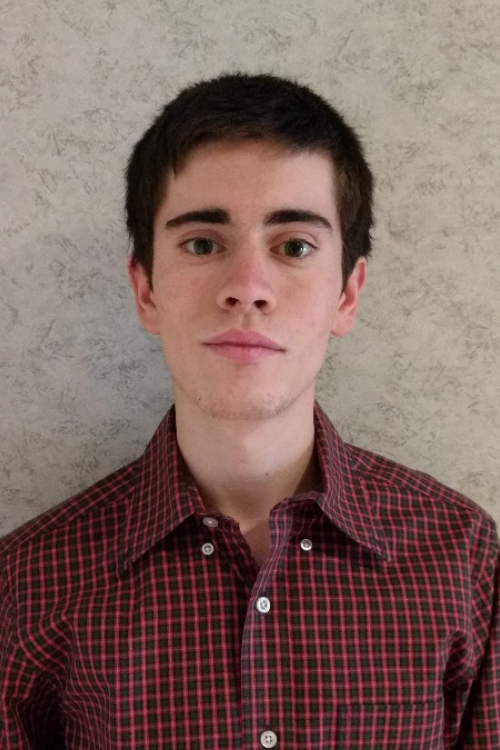
\includegraphics[scale=0.20]{fotoCV}}
\end{picture}

\thispagestyle{onlyfooter}

\makecvtitle
\addtolength{\parskip}{6pt}

\section{\spa{Experiencia Laboral}\en{Work Experience}}

\cventry
    {\spa{Abril 2018--Presente}\en{April 2018--Now}}
    {\spa{Desarrollador de software}\en{Software developer}}
    {Raico S.A. \normalfont - \spa{Importación y exportación aérea y marítima.} \en{Air shipment and ocean freight services.}}{}{}{\url{https://www.raiconet.com/}
    \begin{itemize}
        \item \spa{Mantenimiento y desarrollo de la aplicación mobile y de la aplicación web Raiconet} \en{Development and support of the web application and the mobile app of Raico S.A.}
        \item \spa{Desarrollo de Exporta Simple, una plataforma web integrada con el Ministerio de Producción y Trabajo de Argentina} \en{Development of \textit{Exporta Simple}, a web platform integrated with the Argentine Ministry of Production}
        \item \spa{Tecnologías utilizadas: Grails, Java, Groovy, MySQL} \en{Technologies: Grails, Java, Groovy, MySQL}
    \end{itemize}
    }

\cventry
    {\spa{Enero 2019--Presente}\en{January 2019--Now}}
    {\spa{Colaborador - Teoría de Algoritmos I - Curso Wachenchauzer}\en{Teaching assistant - Algorithm Theory I}}
    {Universidad de Buenos Aires, Facultad de Ingeniería}{}{}{\url{https://algoritmos-rw.github.io/tda/}
    \begin{itemize}
        \item \spa{Clases prácticas, talleres, preparación y corrección de exámenes.} \en{Classes, workshops, making and grading of exams.}
        \item \spa{Temas cubiertos: Complejidad computacional (notación $\mathcal{O}, \Theta, \Omega$, clases de problemas P, NP), paradigmas de diseño algorítmico y heurísticas (división y conquista, técnicas greedy, programación dinámica)} \en{Covered topics: Complexity ($\mathcal{O}, \Theta, \Omega$ notation and P, NP classes), algorithm design and heuristics (divide and conquer, dynamic programming, greedy techniques).}
    \end{itemize}
    }
\vspace{-2em}
\cventry
    {\spa{Agosto 2017--Presente}\en{August 2017--Now}}
    {\spa{Colaborador - Algoritmos y Programación II - Curso Wachenchauzer}\en{Teaching assistant - Algorithms and Programming II}}
    {}{}{}{\url{https://algoritmos-rw.github.io/algo2/}
    \begin{itemize}
        \item \spa{Clases prácticas, talleres, preparación y corrección de exámenes.} \en{Classes, workshops, making and grading of exams.}
        \item \spa{Temas cubiertos: C, manejo de memoria, complejidad algorítmica, tipo de datos abstractos, estructuras de datos (listas enlazadas, tablas de hash, árboles, colas de prioridad), teoría de grafos (árboles de tendidos mínimos, recorridos)} \en{Covered topics: C, memory management, algorithmic complexity, abstract data types, data structures (linked lists, hash tables, trees, heap queues), graph theory (minimum spanning tree, traversal).}
    \end{itemize}
    }

\section{\spa{Educación}\en{Education}}

\cventry
    {\spa{2016--Presente}\en{2016--Now}}
    {\spa{Estudiante de Ingeniería en Informática}\en{Computer Engineering student}}
    {Universidad de Buenos Aires, Facultad de Ingeniería}{}{}{
        \spa{Calificaciones distinguidas}\en{Distinguished grades}:
        \begin{itemize}
            \item \spa{Organización de Datos - Sobresaliente (10)} \en{Data Organization - Outstanding (10)}
            \item \spa{Teoría de Algoritmos I - Sobresaliente (10)} \en{Algorithm Theory I - Outstanding (10)}
            \item \spa{Sistemas Operativos - Sobresaliente (10)} \en{Operating Systems - Outstanding (10)}
            \item \spa{Álgebra - Distinguido (9)} \en{Algebra - Distinguished (9)}
            \item \spa{Algoritmos y Programación II - Distinguido (9)} \en{Algorithms and Programming II - Distinguished (9)}
            \item \spa{Algoritmos y Programación I - Distinguido (8)} \en{Algorithms and Programming I - Distinguished (8)}
        \end{itemize}
    }

\cventry
    {2009--2014}
    {\spa{Bachiller Bilingüe en Economía y Administración}\en{Bilingual bachelors' degree in economics and business administration}}
    {Colegio Ward}{}{}{\textit{\spa{Promedio general}\en{Grade Point Average} 8.29}}

% \cventry
%     {2012--2013}
%     {International General Certificate of Secondary Education (IGCSE)}
%     {University of Cambridge}{}{}{\textit{Passed with Merit}}
%     Environmental Management B
%     Geography B
%     First Language Spanish D
%     Economics B
%     Mathematics B
%     Business Studies C
%     First language english D

% \cventry
%     {2011}
%     {First Certificate in English}
%     {University of Cambridge}{}{}{\textit{Grade C}}
% Cambridge ESOL Level 1 Certificate in ESOL International

\section{\spa{Conocimientos específicos}\en{Specific skills}}

\begin{itemize}
\item \textbf{\spa{Lenguajes de programación}\en{Programming languages}:} C, Python, Java, JavaScript.

\item \textbf{\spa{Paradigmas de programación y técnicas de diseño de algoritmos}\en{Programming paradigms and algorithm design techniques}:} 
    \spa{Programación procedural, programación orientada a objetos, programación dinámica, división y conquista, metodologías greedy}\en{Procedural programming, object-oriented programming, dynamic programming, divide and conquer, greedy algorithms}

\item \textbf{\spa{Otros tópicos}\en{Other topics}:}
    \spa{Análisis de datos, complejidad computacional, machine learning, MapReduce, teoría de grafos, compresión de datos, PageRank, hashing}
    \en{Data analysis, computational complexity, machine learning, MapReduce, graph theory, data compression, PageRank, hashing}

\item \textbf{\spa{Otros lenguajes}\en{Other languages}:} SQL, TeX.

\item \textbf{\spa{Frameworks y otros}\en{Frameworks and miscellaneous}:} Groovy, Grails, Pandas, PySpark.

\end{itemize}

\IfFileExists{./notas.pdf}{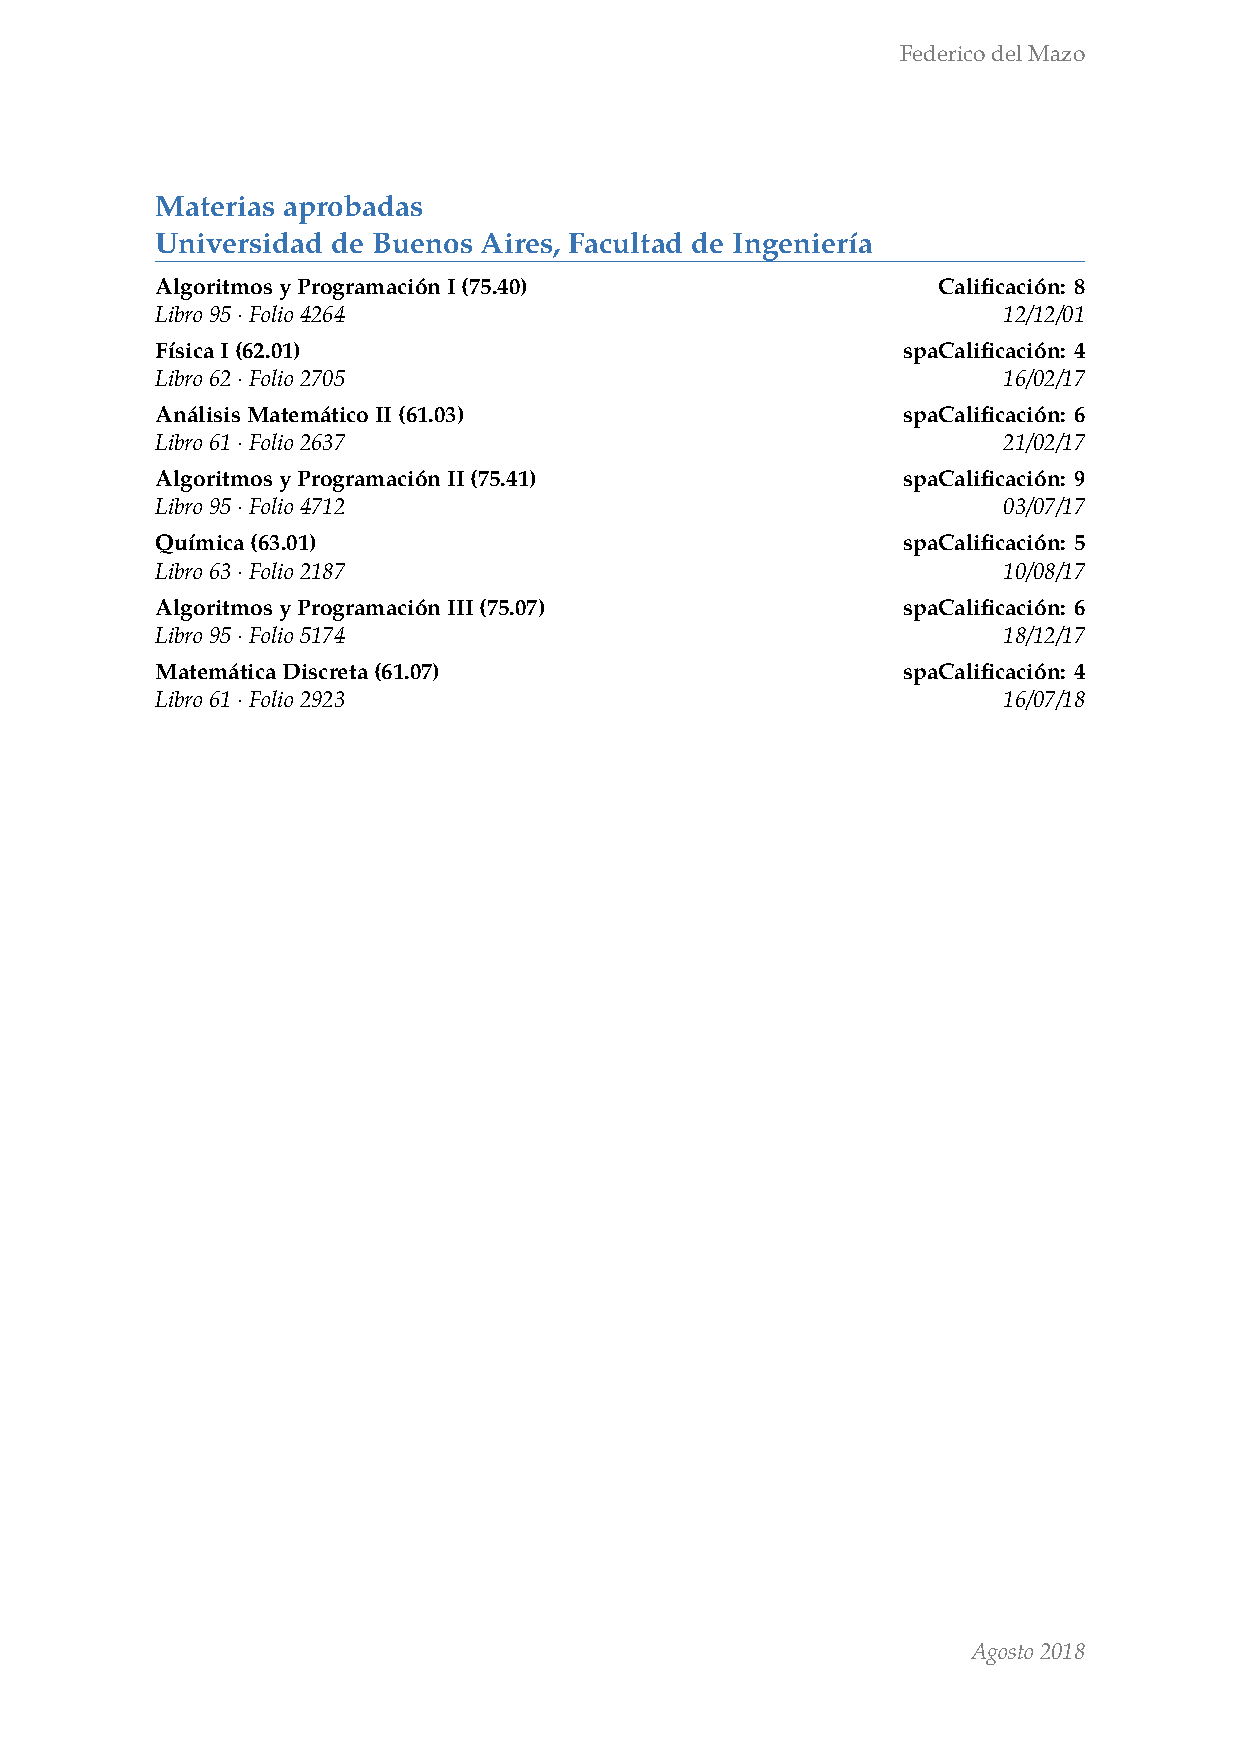
\includepdf[pages=-]{notas.pdf}}{}
\end{document}

